\documentclass{article}

\usepackage[dblblindworkshop, final]{neurips_2026}
\workshoptitle{Foundation Models for Temporal Systems}

\usepackage[utf8]{inputenc}
\usepackage[T1]{fontenc}
\usepackage{hyperref}
\usepackage{url}
\usepackage{booktabs}
\usepackage{amsfonts}
\usepackage{amsmath}
\usepackage{amssymb}
\usepackage{nicefrac}
\usepackage{microtype}
\usepackage{xcolor}
\usepackage{graphicx}
\renewcommand{\ttdefault}{lmtt}
\hypersetup{pdftitle={Position and Elapsed Time in Sparse-Time Probes of Time Series Foundation Models},pdfauthor={Akanksha Gupta}}

\newcommand{\mperp}{m^{\perp}}
\newcommand{\dt}{\Delta t}

\title{Position and Elapsed Time in Sparse-Time Probes of Time Series Foundation Models}

\author{%
  Akanksha Gupta\\
  3am Labs\\
  \texttt{akanksha@3amlabs.ai}
}

\begin{document}

\maketitle

\begin{abstract}
Time series foundation models (TSFMs) are often applied to series with missing observations by dropping the missing steps and passing the remaining values in order, so that the 40th token may be the 40th reading or the 400th.
Linear probes are a natural way to ask whether the hidden states still reflect elapsed time, but we show that a straightforward probing protocol gives the wrong answer.
Under a skewed keep law, elapsed time remains a nonlinear function of token position after its linear trend is removed, and the probe recovers it from white noise; under random dropout and block outages, shuffled folds within a series let the probe interpolate a smooth target, again from white noise.
Held-out series, matched-keep white noise, and a position-only oracle separate the two failures.
On eight TSFMs and 102 UCR series, we find that every model encodes token position from white noise ($r \ge 0.94$), and that the planned gap test passes for most models but at about the level of a probe on local value changes that uses no model.
Where the values reveal the gaps, ridge probes recover elapsed time at $r = 0.44$--$0.63$, while a running sum of that no-model gap probe does better.
We do not evaluate forecasts.
\end{abstract}

\section{Introduction}
\label{sec:intro}

Real-world series are frequently irregular: a sensor may stop reporting when it saturates, and a metrics pipeline may go silent during an outage.
A common way to apply a pretrained forecaster is to drop the missing steps and pass the observed values in order, because the data have no regular grid, as in event logs, or because the pipeline removes gaps before the model call.
Models designed for irregular series instead take a mask or the observation times as input~\citep{che2018grud,rubanova2019latent,kidger2020ncde,shukla2021mtan}, and Chronos-T5, Chronos-Bolt, and Chronos-2 can all accept NaNs on the original grid; here we study the dropped input.

Because elapsed time rises with token position, a probe can score well simply by reading position, and the usual remedy is to remove the linear trend in position from the target.
This leaves two failures (the ``dual collinearity'' of the original version).
First, a skewed keep law makes elapsed time a smooth nonlinear function of rank, and that curve survives the linear correction.
Second, with shuffled folds inside a series, a test token's neighbours usually sit in the training folds, so any representation that varies smoothly along the sequence can interpolate a smooth target.
In both cases the probe decodes elapsed time from white noise.
A probe result is only meaningful against a control that the probe can solve without the property of interest~\citep{hewitt2019control}, and the same separation is required before a hippocampal cell is said to encode time rather than distance~\citep{kraus2013time}.

Linear probes, which regress a property on hidden states and score the held-out correlation~\citep{alain2017understanding,tenney2019bert,belinkov2022probing}, have been used on TSFMs to study trend, periodicity, and other temporal factors~\citep{wilinski2024exploring,pandey2025internal} and dataset-level sampling cadence~\citep{mavani2026observability}, the latter already with series-disjoint splits and probes on the raw input.
We know of no published study that probes elapsed time under missing observations with shuffled folds inside each series, and we do not claim that this protocol is established practice: the first version of this analysis used it, on Chronos-T5-base and eight series, and its correlations on real data were close to those on white noise.
The rest of the paper applies the controls above to the wider set of models, series, and missingness patterns requested in review.

\section{Setup}
\label{sec:setup}

\textbf{Models.}
We probe frozen public weights at every layer, including the input embedding.
Chronos-T5 (tiny through large; \citealp{ansari2024chronos}) is a T5 encoder-decoder~\citep{raffel2020t5} with one quantized token per step and relative attention biases, so its input embedding carries no absolute position; we read the encoder and report all five sizes, where the original audit used only base.
Chronos-Bolt-base~\citep{chronosbolt} follows the same design over left-padded patches of 16 steps, and Chronos-2~\citep{ansari2025chronos2} is an encoder over the same patches in which each step carries a mask and a time index measured in units of the maximum context length.
Time-MoE-50M~\citep{shi2025timemoe} is a causal decoder with one token per step, rotary embeddings, and no NaN handling.
Every model receives only the kept values, in order.

\textbf{Data and missingness.}
We take the first training series of each UCR 2018 dataset~\citep{dau2019ucr}, truncate it to 512 steps, keep the 102 series that are at least 128 steps long with non-zero variance, and $z$-score them; this rule was fixed before any model was run.
The first and last steps are always kept.
Random dropout keeps $n = \mathrm{round}((1-p)T)$ steps chosen completely at random~\citep{little2019missing}.
Block outages alternate observed and missing runs of geometric length with a mean outage of 10 steps, so the missing rate is $p$ in expectation and the number of kept steps varies by draw; a draw that keeps fewer than eight points is replaced by a random-dropout draw.
Value-dependent missingness, added after the analysis plan, chooses a fixed number of interior steps to drop, sampled without replacement with weight proportional to $\exp(1.5 z_t)$.
The Beta keep of the original audit truncates $\mathrm{Beta}(0.35,4)\cdot(T-1)$ toward zero and keeps the first $n-2$ distinct interior times, so that at $p = 0.5$ about 83\% of its gaps are a single step.
Each series is also paired with standard normal noise at the same kept steps.
Section~\ref{sec:trap} uses four drop rates and one draw; Section~\ref{sec:ladder} uses $p \in \{0.5, 0.7\}$ and three draws, averaged per series before taking the median.

\textbf{Targets and probes.}
We probe three targets: token position $k$; elapsed time $\mperp$, the normalized observation time with its linear trend in $k$ removed; and the gap $\dt$ between consecutive kept steps.
For patch models these become the patch index, the time of the patch's last observation, and the time elapsed since the previous patch ended, with the first patch measured from $t = 0$; our main sweep instead averaged the step-level targets within each patch, so Bolt's result on that older target is not comparable to Table~\ref{tab:main}.
Our primary probes fit a ridge regression ($\lambda = 1$) per target on held-out series, using five folds grouped by series and states standardized within the training fold, and we report the median Pearson $r$ over series.
Shuffled and contiguous folds within a series follow the original protocol, fitting ridge on the raw states and averaging the fold correlations; contiguous folds hold out one block at a time, although interior blocks still sit between training tokens.
As an exploratory check we also fit an MLP with two hidden layers of 256 units and one joint head for position, gap, and elapsed time, using the same folds with early stopping on 15\% of the training series, and we run it on the white-noise inputs as well.

\begin{figure}[ht]
  \centering
  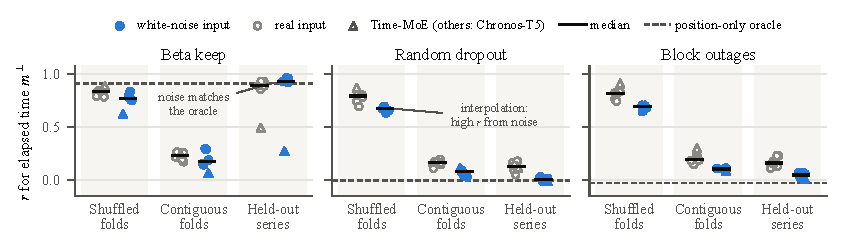
\includegraphics[width=\linewidth]{figures/fig1_trap.pdf}
  \caption{Final-layer $r$ for $\mperp$ at $p = 0.5$ for Chronos-T5 (circles) and Time-MoE (triangles), from white noise (filled) and real data (open); the dashed line is the position-only oracle.
  Under random dropout and block outages, where the oracle is about 0, shuffled folds still read $r = 0.63$--$0.71$ from noise.}
  \label{fig:trap}
\end{figure}

\textbf{Reference baselines.}
These references are not ceilings: the position-only oracle is the Monte Carlo expectation of the target given position.
The difference probe applies the same held-out split to local input features: a five-point window and its differences for the encoders, past values only for Time-MoE, and within-patch summaries for the patch models.
The running sum accumulates the difference probe's gap estimates and is then residualized on position in the same way as $\mperp$.
The difference probe, the running sum, the MLP, and the additional draws were also added after the analysis plan.
Table~\ref{tab:main} selects its layer on 30\% of the series and reports results on the remaining 71, while Section~\ref{sec:trap} and the replication of the original eight-series numbers (Appendix~\ref{app:replication}) use the final layer.

\section{Elapsed time from white noise}
\label{sec:trap}


Under the Beta keep, $\mperp$ remains a smooth function of rank.
Held-out probes on Chronos-T5 read it from white noise at $r = 0.92$--$0.97$, against a position-only oracle of 0.92 (final layer), and Chronos-Bolt and Chronos-2 reach 0.96--0.97 against a patch-level oracle of 0.997 (main sweep, per-patch averages, best layer).
Time-MoE is the exception (0.27): in a causal decoder a token cannot see how many tokens follow it, while the Beta curve depends on rank within the whole window.

Under random dropout and block outages the oracle is close to 0, and held-out probes recover essentially nothing from noise ($r \le 0.07$).
Shuffled folds, which we ran for the six one-token models, nevertheless report $r = 0.63$--$0.71$ from white noise at $p = 0.5$ and $0.70$--$0.91$ on real data, while contiguous folds fall to $0.03$--$0.12$~\citep{bergmeir2012cv,roberts2017cv}.
Shuffled folds therefore measure smoothness along the series; held-out series remove that interpolation, and the white-noise input and the oracle expose the remaining position geometry.

\section{What the corrected probes recover}
\label{sec:ladder}

\begin{figure}[ht]
  \centering
  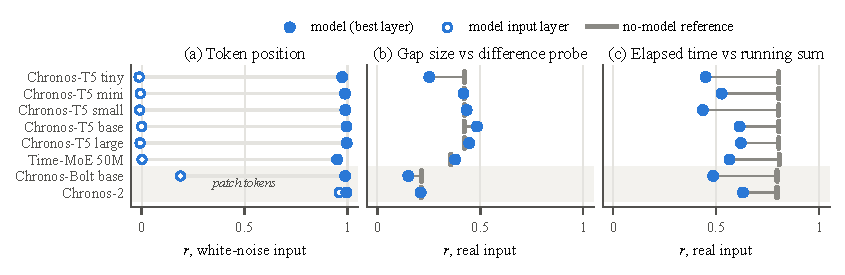
\includegraphics[width=\linewidth]{figures/fig2_v2.pdf}
  \caption{Held-out ridge probes averaged over three draws.
  (a)~Token position from white noise under random dropout at $p = 0.5$; open marks show the input layer.
  (b)~Gap $\dt$ on real data at the same rate, with grey ticks marking the difference probe.
  (c)~Elapsed time under value-dependent missingness at $p = 0.7$, with grey ticks marking the running sum.}
  \label{fig:ladder}
\end{figure}

\begin{table}[ht]
  \caption{Held-out ridge probes, with the layer chosen on 30\% of series.
  Position is $r(k)$ from white noise; Gap is the real-minus-noise $\Delta r$ for $\dt$ under random dropout at $p = 0.5$, with a 95\% interval.
  The last three columns give the model minus the difference probe for $\dt$ in the same condition, and the model minus the running sum for $\mperp$ at $p = 0.7$.
  A star marks an interval that excludes 0; MLP pairs are in Appendix~\ref{app:pairs}.}
  \label{tab:main}
  \centering
  \small
  \setlength{\tabcolsep}{3.5pt}
  \begin{tabular}{lccccc}
    \toprule
    Model & Position & Gap $\Delta r$ [95\% CI] & vs difference probe & Block & Value-dependent \\
    \midrule
    Chronos-T5 tiny (8M) & 0.974 & 0.25 [0.21, 0.30] & $-0.12^{\ast}$ & $-0.17^{\ast}$ & $-0.27^{\ast}$ \\
    Chronos-T5 mini (20M) & 0.988 & 0.40 [0.30, 0.47] & $-0.00$ & $-0.11^{\ast}$ & $-0.20^{\ast}$ \\
    Chronos-T5 small (46M) & 0.990 & 0.41 [0.33, 0.49] & $+0.04^{\ast}$ & $-0.11^{\ast}$ & $-0.24^{\ast}$ \\
    Chronos-T5 base (200M) & 0.995 & 0.48 [0.36, 0.57] & $+0.06^{\ast}$ & $-0.10^{\ast}$ & $-0.17^{\ast}$ \\
    Chronos-T5 large (710M) & 0.996 & 0.44 [0.34, 0.51] & $+0.03^{\ast}$ & $-0.14^{\ast}$ & $-0.15^{\ast}$ \\
    Time-MoE (50M) & 0.950 & 0.39 [0.33, 0.45] & $+0.01$ & $-0.17^{\ast}$ & $-0.18^{\ast}$ \\
    Chronos-Bolt base & 0.989 & 0.05 [$-0.06$, 0.08] & $-0.06^{\ast}$ & $-0.14^{\ast}$ & $-0.25^{\ast}$ \\
    Chronos-2 & 0.994 & 0.13 [0.02, 0.16] & $-0.08^{\ast}$ & $-0.20^{\ast}$ & $-0.09^{\ast}$ \\
    \bottomrule
  \end{tabular}
\end{table}

Every model decodes token position from white noise at $r = 0.94$--$0.996$, and across Chronos-T5 sizes from 8M to 710M parameters this rises from 0.974 to 0.996.
For Chronos-T5 and Time-MoE the input embedding carries no position and it appears within the first few layers, whereas Chronos-2's input embedding already reaches about 0.96 through its time index on the shortened series.

The analysis plan, written before the runs and released with the code, defined the gap test as decoding $\dt$ under random dropout at $p = 0.5$, with a median real-minus-noise $\Delta r$ above 0.10 and an interval that excludes 0.
On the planned draw, seven models passed and Chronos-2 did not.
Averaged over three draws, the six one-token models still pass (gap $\Delta r$ rises from 0.25 at Chronos-T5 tiny to 0.40 at mini and then flattens) and Chronos-2 now passes as well, at 0.13 [0.02, 0.16]; Chronos-Bolt, which passed the planned draw under the old per-patch averages, gives 0.05 [$-0.06$, 0.08] under the last-observation target in Table~\ref{tab:main}.

The gap signal is largely what the input already shows: a difference probe on local value changes reaches $r = 0.42$ in the same condition (0.36 with past values only); Chronos-T5 mini and Time-MoE match it, tiny falls short by 0.12, and Chronos-T5 small through large sit 0.03--0.06 above it, comparable to the draw-to-draw movement of the medians (about $\pm 0.05$).
Across series, the gap result also tracks lag-1 autocorrelation (Spearman $\rho = 0.52$--$0.70$ for the one-token models): a jump between values signals elapsed time mainly when the series is smooth.

Under random dropout at $p = 0.7$, elapsed time is barely decodable: model correlations are about 0.10--0.23 and the running sum reaches about 0.13--0.25.
Five of eight ridge intervals exclude zero and are negative, Chronos-2's ridge difference is $+0.06$ with an interval that includes zero, and most MLP intervals include zero.
Under block outages, ridge correlations are about 0.14--0.27 and every model in Table~\ref{tab:main} falls below the running sum.
Under value-dependent missingness, where large jumps in value mark large gaps, ridge correlations rise to $0.44$--$0.63$, but the running sum reaches about 0.80.
The same deficit holds at $p = 0.5$ for all 32 model--probe pairs, with intervals excluding zero (Appendix~\ref{app:pairs}).
The comparison is not symmetric, since the running sum has an explicit accumulator while the probe must find accumulated time in one token's state; the deficit shows that these probes do not read it out in that form.
On white noise, the MLP decodes essentially no elapsed time for the one-token models ($|r| \le 0.071$ in every condition).

\section{Recommendations and limitations}
\label{sec:recs}
\label{sec:limits}

When probing elapsed time in a sequence model with missing observations, we recommend (1)~running the probe on white noise at the same kept steps; (2)~evaluating on held-out series; (3)~reporting the position-only oracle, since a model that matches it is reading position; (4)~probing gaps and elapsed time separately; and (5)~comparing against a no-model baseline built from the features the model is claimed to use, where a baseline that sums the gaps tests whether the states expose that sum.

Value-dependent missingness is only one missing-not-at-random mechanism, and UCR series are short and univariate.
We measure representations rather than forecasts.
Quantizing the difference probe's inputs as Chronos-T5 does changes the model-minus-probe gap correlations by at most 0.015.
We also do not evaluate the NaN-on-grid input that the three Chronos models accept.

\section{Conclusion}
\label{sec:conc}

With held-out series, matched-keep white noise, and a position-only oracle as controls, every model we tested encodes token position from noise, the one-token models decode gaps about as well as a no-model probe on local value changes, and where the values reveal the gaps, that probe's running sum recovers more elapsed time than the states do.
Whether the Chronos models use the spacing when missing steps stay on the grid is untested.
Code and per-series results: \url{https://github.com/AIpsychonaut/neurips-fmts-2026}.

\begin{ack}
No external funding was received for this work.
The author declares no competing interests.
\end{ack}

{\small
\bibliographystyle{plainnat}
\bibliography{refs}
}

\appendix

\section{Protocol}
\label{app:protocol}

Chronos-T5 states are the encoder hidden states after the model's own tokenizer, with the EOS position dropped.
Chronos-Bolt states are the encoder states on left-padded patches; the register token appended by the model is dropped before probing.
Chronos-2's \texttt{encode} in \texttt{chronos-forecasting}~2.3.2 embeds the context patches and one future query patch, joins them, and runs the encoder once; our hooks keep the context rows.
Time-MoE states are the inner decoder's hidden states on values $z$-scored per series.
In \texttt{chronos-forecasting}~2.3.2, a NaN left on the grid keeps its slot in all three Chronos models: Chronos-T5 masks it as a padding token, while Bolt and Chronos-2 mark it in the mask channel, and Chronos-2's time index still counts it.
Seeds are $42 + 1000s + 100\ell + \mathrm{round}(10p)$ plus $10^{7}$ times the draw index, and the noise input adds $7777777$.
The oracle uses 200 Monte Carlo draws and 50 rank bins, and patch-model medians omit series with fewer than eight patches (about 22\% of cells).
Compute was about 5 GPU-hours in total on NVIDIA A10G GPUs, one per model.

\section{Replication}
\label{app:replication}

On the original eight series, truncated at 400, with the Beta keep at $p = 0.5$, Chronos-T5-base, the final layer, and shuffled folds, the pipeline gives a median $r(\mperp)$ of 0.821 on real data in both bf16 and fp32.
On noise it gives 0.760 in bf16 (0.7597 before rounding) and 0.759 in fp32, against 0.821 and 0.759 in the submitted version.

\section{Further pairs}
\label{app:pairs}

Table~\ref{tab:appc} reports the model minus the running sum for $\mperp$ at $p = 0.7$ under ridge and MLP probes; every interval excludes 0.
At $p = 0.5$, all 32 model--probe pairs also fall below the running sum with intervals excluding 0.
These intervals are series bootstraps for one comparison at a time and are not adjusted for the number of models and conditions.
Full grids are released with the code.

\begin{table}[h]
  \caption{Model minus running sum at $p = 0.7$, ridge / MLP.}
  \label{tab:appc}
  \centering
  \small
  \begin{tabular}{lcc}
    \toprule
    Model & Block outages & Value-dependent \\
    \midrule
    Chronos-T5 tiny & $-0.17^{\ast}$ / $-0.25^{\ast}$ & $-0.27^{\ast}$ / $-0.26^{\ast}$ \\
    Chronos-T5 mini & $-0.11^{\ast}$ / $-0.21^{\ast}$ & $-0.20^{\ast}$ / $-0.18^{\ast}$ \\
    Chronos-T5 small & $-0.11^{\ast}$ / $-0.22^{\ast}$ & $-0.24^{\ast}$ / $-0.24^{\ast}$ \\
    Chronos-T5 base & $-0.10^{\ast}$ / $-0.18^{\ast}$ & $-0.17^{\ast}$ / $-0.16^{\ast}$ \\
    Chronos-T5 large & $-0.14^{\ast}$ / $-0.15^{\ast}$ & $-0.15^{\ast}$ / $-0.13^{\ast}$ \\
    Time-MoE & $-0.17^{\ast}$ / $-0.22^{\ast}$ & $-0.18^{\ast}$ / $-0.23^{\ast}$ \\
    Chronos-Bolt & $-0.14^{\ast}$ / $-0.14^{\ast}$ & $-0.25^{\ast}$ / $-0.07^{\ast}$ \\
    Chronos-2 & $-0.20^{\ast}$ / $-0.15^{\ast}$ & $-0.09^{\ast}$ / $-0.10^{\ast}$ \\
    \bottomrule
  \end{tabular}
\end{table}

\newpage
\section*{NeurIPS Paper Checklist}



\begin{enumerate}

\item {\bf Claims}
    \item[] Question: Do the main claims made in the abstract and introduction accurately reflect the paper's contributions and scope?
    \item[] Answer: \answerYes{}
    \item[] Justification: The abstract and \S\ref{sec:intro} state the claims, which \S\ref{sec:trap} and \S\ref{sec:ladder} support. Analyses added after the analysis plan are labelled as such.
    \item[] Guidelines:
    \begin{itemize}
        \item The answer \answerNA{} means that the abstract and introduction do not include the claims made in the paper.
        \item The abstract and/or introduction should clearly state the claims made, including the contributions made in the paper and important assumptions and limitations. A \answerNo{} or \answerNA{} answer to this question will not be perceived well by the reviewers. 
        \item The claims made should match theoretical and experimental results, and reflect how much the results can be expected to generalize to other settings. 
        \item It is fine to include aspirational goals as motivation as long as it is clear that these goals are not attained by the paper. 
    \end{itemize}

\item {\bf Limitations}
    \item[] Question: Does the paper discuss the limitations of the work performed by the authors?
    \item[] Answer: \answerYes{}
    \item[] Justification: \S\ref{sec:limits}.
    \item[] Guidelines:
    \begin{itemize}
        \item The answer \answerNA{} means that the paper has no limitation while the answer \answerNo{} means that the paper has limitations, but those are not discussed in the paper. 
        \item The authors are encouraged to create a separate ``Limitations'' section in their paper.
        \item The paper should point out any strong assumptions and how robust the results are to violations of these assumptions (e.g., independence assumptions, noiseless settings, model well-specification, asymptotic approximations only holding locally). The authors should reflect on how these assumptions might be violated in practice and what the implications would be.
        \item The authors should reflect on the scope of the claims made, e.g., if the approach was only tested on a few datasets or with a few runs. In general, empirical results often depend on implicit assumptions, which should be articulated.
        \item The authors should reflect on the factors that influence the performance of the approach. For example, a facial recognition algorithm may perform poorly when image resolution is low or images are taken in low lighting. Or a speech-to-text system might not be used reliably to provide closed captions for online lectures because it fails to handle technical jargon.
        \item The authors should discuss the computational efficiency of the proposed algorithms and how they scale with dataset size.
        \item If applicable, the authors should discuss possible limitations of their approach to address problems of privacy and fairness.
        \item While the authors might fear that complete honesty about limitations might be used by reviewers as grounds for rejection, a worse outcome might be that reviewers discover limitations that aren't acknowledged in the paper. The authors should use their best judgment and recognize that individual actions in favor of transparency play an important role in developing norms that preserve the integrity of the community. Reviewers will be specifically instructed to not penalize honesty concerning limitations.
    \end{itemize}

\item {\bf Theory assumptions and proofs}
    \item[] Question: For each theoretical result, does the paper provide the full set of assumptions and a complete (and correct) proof?
    \item[] Answer: \answerNA{}
    \item[] Justification: The paper has no theoretical results.
    \item[] Guidelines:
    \begin{itemize}
        \item The answer \answerNA{} means that the paper does not include theoretical results. 
        \item All the theorems, formulas, and proofs in the paper should be numbered and cross-referenced.
        \item All assumptions should be clearly stated or referenced in the statement of any theorems.
        \item The proofs can either appear in the main paper or the supplemental material, but if they appear in the supplemental material, the authors are encouraged to provide a short proof sketch to provide intuition. 
        \item Inversely, any informal proof provided in the core of the paper should be complemented by formal proofs provided in appendix or supplemental material.
        \item Theorems and Lemmas that the proof relies upon should be properly referenced. 
    \end{itemize}

    \item {\bf Experimental result reproducibility}
    \item[] Question: Does the paper fully disclose all the information needed to reproduce the main experimental results of the paper to the extent that it affects the main claims and/or conclusions of the paper (regardless of whether the code and data are provided or not)?
    \item[] Answer: \answerYes{}
    \item[] Justification: \S\ref{sec:setup} and Appendix~\ref{app:protocol} give the models, data selection, missingness patterns, seeds, probes and references. All weights and data are public.
    \item[] Guidelines:
    \begin{itemize}
        \item The answer \answerNA{} means that the paper does not include experiments.
        \item If the paper includes experiments, a \answerNo{} answer to this question will not be perceived well by the reviewers: Making the paper reproducible is important, regardless of whether the code and data are provided or not.
        \item If the contribution is a dataset and\slash or model, the authors should describe the steps taken to make their results reproducible or verifiable. 
        \item Depending on the contribution, reproducibility can be accomplished in various ways. For example, if the contribution is a novel architecture, describing the architecture fully might suffice, or if the contribution is a specific model and empirical evaluation, it may be necessary to either make it possible for others to replicate the model with the same dataset, or provide access to the model. In general. releasing code and data is often one good way to accomplish this, but reproducibility can also be provided via detailed instructions for how to replicate the results, access to a hosted model (e.g., in the case of a large language model), releasing of a model checkpoint, or other means that are appropriate to the research performed.
        \item While NeurIPS does not require releasing code, the conference does require all submissions to provide some reasonable avenue for reproducibility, which may depend on the nature of the contribution. For example
        \begin{enumerate}
            \item If the contribution is primarily a new algorithm, the paper should make it clear how to reproduce that algorithm.
            \item If the contribution is primarily a new model architecture, the paper should describe the architecture clearly and fully.
            \item If the contribution is a new model (e.g., a large language model), then there should either be a way to access this model for reproducing the results or a way to reproduce the model (e.g., with an open-source dataset or instructions for how to construct the dataset).
            \item We recognize that reproducibility may be tricky in some cases, in which case authors are welcome to describe the particular way they provide for reproducibility. In the case of closed-source models, it may be that access to the model is limited in some way (e.g., to registered users), but it should be possible for other researchers to have some path to reproducing or verifying the results.
        \end{enumerate}
    \end{itemize}


\item {\bf Open access to data and code}
    \item[] Question: Does the paper provide open access to the data and code, with sufficient instructions to faithfully reproduce the main experimental results, as described in supplemental material?
    \item[] Answer: \answerYes{}
    \item[] Justification: Code, the analysis plan and per-series results are in the repository linked in \S\ref{sec:conc}. UCR~2018~\citep{dau2019ucr} and the model weights are public.
    \item[] Guidelines:
    \begin{itemize}
        \item The answer \answerNA{} means that paper does not include experiments requiring code.
        \item Please see the NeurIPS code and data submission guidelines (\url{https://neurips.cc/public/guides/CodeSubmissionPolicy}) for more details.
        \item While we encourage the release of code and data, we understand that this might not be possible, so \answerNo{} is an acceptable answer. Papers cannot be rejected simply for not including code, unless this is central to the contribution (e.g., for a new open-source benchmark).
        \item The instructions should contain the exact command and environment needed to run to reproduce the results. See the NeurIPS code and data submission guidelines (\url{https://neurips.cc/public/guides/CodeSubmissionPolicy}) for more details.
        \item The authors should provide instructions on data access and preparation, including how to access the raw data, preprocessed data, intermediate data, and generated data, etc.
        \item The authors should provide scripts to reproduce all experimental results for the new proposed method and baselines. If only a subset of experiments are reproducible, they should state which ones are omitted from the script and why.
        \item At submission time, to preserve anonymity, the authors should release anonymized versions (if applicable).
        \item Providing as much information as possible in supplemental material (appended to the paper) is recommended, but including URLs to data and code is permitted.
    \end{itemize}


\item {\bf Experimental setting/details}
    \item[] Question: Does the paper specify all the training and test details (e.g., data splits, hyperparameters, how they were chosen, type of optimizer) necessary to understand the results?
    \item[] Answer: \answerYes{}
    \item[] Justification: \S\ref{sec:setup} and Appendix~\ref{app:protocol}: ridge $\lambda=1$, five folds grouped by series, layer selection on a fixed 30\% of series.
    \item[] Guidelines:
    \begin{itemize}
        \item The answer \answerNA{} means that the paper does not include experiments.
        \item The experimental setting should be presented in the core of the paper to a level of detail that is necessary to appreciate the results and make sense of them.
        \item The full details can be provided either with the code, in appendix, or as supplemental material.
    \end{itemize}

\item {\bf Experiment statistical significance}
    \item[] Question: Does the paper report error bars suitably and correctly defined or other appropriate information about the statistical significance of the experiments?
    \item[] Answer: \answerYes{}
    \item[] Justification: Medians over series with series-bootstrap 95\% intervals (2{,}000 resamples); \S\ref{sec:ladder} averages three missingness draws. Intervals are not adjusted for multiple comparisons (Appendix~\ref{app:pairs}).
    \item[] Guidelines:
    \begin{itemize}
        \item The answer \answerNA{} means that the paper does not include experiments.
        \item The authors should answer \answerYes{} if the results are accompanied by error bars, confidence intervals, or statistical significance tests, at least for the experiments that support the main claims of the paper.
        \item The factors of variability that the error bars are capturing should be clearly stated (for example, train/test split, initialization, random drawing of some parameter, or overall run with given experimental conditions).
        \item The method for calculating the error bars should be explained (closed form formula, call to a library function, bootstrap, etc.)
        \item The assumptions made should be given (e.g., Normally distributed errors).
        \item It should be clear whether the error bar is the standard deviation or the standard error of the mean.
        \item It is OK to report 1-sigma error bars, but one should state it. The authors should preferably report a 2-sigma error bar than state that they have a 96\% CI, if the hypothesis of Normality of errors is not verified.
        \item For asymmetric distributions, the authors should be careful not to show in tables or figures symmetric error bars that would yield results that are out of range (e.g., negative error rates).
        \item If error bars are reported in tables or plots, the authors should explain in the text how they were calculated and reference the corresponding figures or tables in the text.
    \end{itemize}

\item {\bf Experiments compute resources}
    \item[] Question: For each experiment, does the paper provide sufficient information on the computer resources (type of compute workers, memory, time of execution) needed to reproduce the experiments?
    \item[] Answer: \answerYes{}
    \item[] Justification: Appendix~\ref{app:protocol}: about 5 GPU-hours in total on NVIDIA A10G GPUs, one per model; probes on CPU.
    \item[] Guidelines:
    \begin{itemize}
        \item The answer \answerNA{} means that the paper does not include experiments.
        \item The paper should indicate the type of compute workers CPU or GPU, internal cluster, or cloud provider, including relevant memory and storage.
        \item The paper should provide the amount of compute required for each of the individual experimental runs as well as estimate the total compute. 
        \item The paper should disclose whether the full research project required more compute than the experiments reported in the paper (e.g., preliminary or failed experiments that didn't make it into the paper). 
    \end{itemize}
    
\item {\bf Code of ethics}
    \item[] Question: Does the research conducted in the paper conform, in every respect, with the NeurIPS Code of Ethics \url{https://neurips.cc/public/EthicsGuidelines}?
    \item[] Answer: \answerYes{}
    \item[] Justification: The work audits public models on a public archive and involves no human subjects.
    \item[] Guidelines:
    \begin{itemize}
        \item The answer \answerNA{} means that the authors have not reviewed the NeurIPS Code of Ethics.
        \item If the authors answer \answerNo, they should explain the special circumstances that require a deviation from the Code of Ethics.
        \item The authors should make sure to preserve anonymity (e.g., if there is a special consideration due to laws or regulations in their jurisdiction).
    \end{itemize}


\item {\bf Broader impacts}
    \item[] Question: Does the paper discuss both potential positive societal impacts and negative societal impacts of the work performed?
    \item[] Answer: \answerNA{}
    \item[] Justification: The paper studies evaluation methodology for model analysis and has no deployment.
    \item[] Guidelines:
    \begin{itemize}
        \item The answer \answerNA{} means that there is no societal impact of the work performed.
        \item If the authors answer \answerNA{} or \answerNo, they should explain why their work has no societal impact or why the paper does not address societal impact.
        \item Examples of negative societal impacts include potential malicious or unintended uses (e.g., disinformation, generating fake profiles, surveillance), fairness considerations (e.g., deployment of technologies that could make decisions that unfairly impact specific groups), privacy considerations, and security considerations.
        \item The conference expects that many papers will be foundational research and not tied to particular applications, let alone deployments. However, if there is a direct path to any negative applications, the authors should point it out. For example, it is legitimate to point out that an improvement in the quality of generative models could be used to generate Deepfakes for disinformation. On the other hand, it is not needed to point out that a generic algorithm for optimizing neural networks could enable people to train models that generate Deepfakes faster.
        \item The authors should consider possible harms that could arise when the technology is being used as intended and functioning correctly, harms that could arise when the technology is being used as intended but gives incorrect results, and harms following from (intentional or unintentional) misuse of the technology.
        \item If there are negative societal impacts, the authors could also discuss possible mitigation strategies (e.g., gated release of models, providing defenses in addition to attacks, mechanisms for monitoring misuse, mechanisms to monitor how a system learns from feedback over time, improving the efficiency and accessibility of ML).
    \end{itemize}
    
\item {\bf Safeguards}
    \item[] Question: Does the paper describe safeguards that have been put in place for responsible release of data or models that have a high risk for misuse (e.g., pre-trained language models, image generators, or scraped datasets)?
    \item[] Answer: \answerNA{}
    \item[] Justification: No data or models with a high risk of misuse are released.
    \item[] Guidelines:
    \begin{itemize}
        \item The answer \answerNA{} means that the paper poses no such risks.
        \item Released models that have a high risk for misuse or dual-use should be released with necessary safeguards to allow for controlled use of the model, for example by requiring that users adhere to usage guidelines or restrictions to access the model or implementing safety filters. 
        \item Datasets that have been scraped from the Internet could pose safety risks. The authors should describe how they avoided releasing unsafe images.
        \item We recognize that providing effective safeguards is challenging, and many papers do not require this, but we encourage authors to take this into account and make a best faith effort.
    \end{itemize}

\item {\bf Licenses for existing assets}
    \item[] Question: Are the creators or original owners of assets (e.g., code, data, models), used in the paper, properly credited and are the license and terms of use explicitly mentioned and properly respected?
    \item[] Answer: \answerYes{}
    \item[] Justification: Chronos, Chronos-Bolt, Chronos-2 and Time-MoE are Apache-2.0 and are cited; the UCR archive is cited and used under its terms.
    \item[] Guidelines:
    \begin{itemize}
        \item The answer \answerNA{} means that the paper does not use existing assets.
        \item The authors should cite the original paper that produced the code package or dataset.
        \item The authors should state which version of the asset is used and, if possible, include a URL.
        \item The name of the license (e.g., CC-BY 4.0) should be included for each asset.
        \item For scraped data from a particular source (e.g., website), the copyright and terms of service of that source should be provided.
        \item If assets are released, the license, copyright information, and terms of use in the package should be provided. For popular datasets, \url{paperswithcode.com/datasets} has curated licenses for some datasets. Their licensing guide can help determine the license of a dataset.
        \item For existing datasets that are re-packaged, both the original license and the license of the derived asset (if it has changed) should be provided.
        \item If this information is not available online, the authors are encouraged to reach out to the asset's creators.
    \end{itemize}

\item {\bf New assets}
    \item[] Question: Are new assets introduced in the paper well documented and is the documentation provided alongside the assets?
    \item[] Answer: \answerYes{}
    \item[] Justification: The released code documents the protocol and regenerates every figure and table.
    \item[] Guidelines:
    \begin{itemize}
        \item The answer \answerNA{} means that the paper does not release new assets.
        \item Researchers should communicate the details of the dataset\slash code\slash model as part of their submissions via structured templates. This includes details about training, license, limitations, etc. 
        \item The paper should discuss whether and how consent was obtained from people whose asset is used.
        \item At submission time, remember to anonymize your assets (if applicable). You can either create an anonymized URL or include an anonymized zip file.
    \end{itemize}

\item {\bf Crowdsourcing and research with human subjects}
    \item[] Question: For crowdsourcing experiments and research with human subjects, does the paper include the full text of instructions given to participants and screenshots, if applicable, as well as details about compensation (if any)? 
    \item[] Answer: \answerNA{}
    \item[] Justification: No crowdsourcing or human subjects.
    \item[] Guidelines:
    \begin{itemize}
        \item The answer \answerNA{} means that the paper does not involve crowdsourcing nor research with human subjects.
        \item Including this information in the supplemental material is fine, but if the main contribution of the paper involves human subjects, then as much detail as possible should be included in the main paper. 
        \item According to the NeurIPS Code of Ethics, workers involved in data collection, curation, or other labor should be paid at least the minimum wage in the country of the data collector. 
    \end{itemize}

\item {\bf Institutional review board (IRB) approvals or equivalent for research with human subjects}
    \item[] Question: Does the paper describe potential risks incurred by study participants, whether such risks were disclosed to the subjects, and whether Institutional Review Board (IRB) approvals (or an equivalent approval/review based on the requirements of your country or institution) were obtained?
    \item[] Answer: \answerNA{}
    \item[] Justification: No human subjects.
    \item[] Guidelines:
    \begin{itemize}
        \item The answer \answerNA{} means that the paper does not involve crowdsourcing nor research with human subjects.
        \item Depending on the country in which research is conducted, IRB approval (or equivalent) may be required for any human subjects research. If you obtained IRB approval, you should clearly state this in the paper. 
        \item We recognize that the procedures for this may vary significantly between institutions and locations, and we expect authors to adhere to the NeurIPS Code of Ethics and the guidelines for their institution. 
        \item For initial submissions, do not include any information that would break anonymity (if applicable), such as the institution conducting the review.
    \end{itemize}

\item {\bf Declaration of LLM usage}
    \item[] Question: Does the paper describe the usage of LLMs if it is an important, original, or non-standard component of the core methods in this research? Note that if the LLM is used only for writing, editing, or formatting purposes and does \emph{not} impact the core methodology, scientific rigor, or originality of the research, declaration is not required.
    %this research? 
    \item[] Answer: \answerNA{}
    \item[] Justification: LLMs are not an important, original, or non-standard component of the core methods. An LLM assistant was used only for coding and writing support under the author's direction, and the author verified all claims, numbers and citations.
    \item[] Guidelines:
    \begin{itemize}
        \item The answer \answerNA{} means that the core method development in this research does not involve LLMs as any important, original, or non-standard components.
        \item Please refer to our LLM policy in the NeurIPS handbook for what should or should not be described.
    \end{itemize}

\end{enumerate}

\end{document}
